\documentclass[12pt,a4paper]{article}
\usepackage[utf8]{inputenc}
\usepackage[OT1]{fontenc}
\usepackage{amsmath}
\usepackage{amsfonts}
\usepackage{amssymb}
\usepackage{graphicx}
\usepackage{tikz}
\usepackage{pgfplotstable}
\usepackage{mathtext}

\usepackage[T1]{fontenc}
\usepackage[utf8]{inputenc}
\usepackage[english, bulgarian, russian]{babel}

\usepackage{tikz}
\usepackage{pgfplots}
\usepackage{indentfirst}
\usepackage[export]{adjustbox}
\usepackage{multirow}
\usepackage{geometry} \geometry{verbose,a4paper,tmargin=2cm,bmargin=2cm,lmargin=1.5cm,rmargin=1.5cm}

\graphicspath{{Images/}}
\usepackage[left=2cm,right=2cm,top=2cm,bottom=2cm]{geometry}
\usepackage{wrapfig}
\usepackage{setspace}
\usepackage{indentfirst}
\usepackage{subfigure}


\begin{document}

\begin{titlepage}
  \begin{center}
    \huge
    Московский Физико-технический Институт
    
    (Национальный исследовательский университет)
    \vspace{0.5cm}

   
    \vspace{0.25cm}
 
    \vfill
 
    \vfill

    \textsc{\bf{Отчет о выполнении работы 3.4.5}}\\[3mm]
    
    {\LARGE Петля гистерезиса (динамический метод)}
  \bigskip
    \vfill
    
\end{center}
\vfill
\begin{flushright}

    Выполнили студентки 2 курса
    
    ФБМФ, группа Б06-103

    Попеску Полина
    
    
    Фитэль Алёна

\end{flushright}
\bigskip


\vfill

\begin{center}
  Долгопрудный, 2022 г.
\end{center}
\end{titlepage}

\section{Введение}


\textbf{Цель работы:} изучение петель гистерезиса различных ферромагнитных
материалов в переменных полях.

\textbf{В работе используются:} автотрансформатор, понижающий
трансформатор, интегрирующая цепочка, амперметр, вольтметр,
электронный осциллограф, делитель напряжения, тороидальные образцы с
двумя обмотками.

\section{Теоретический материал}

Основные характеристики
ферромагнетиков — их коэрцитивное поле $H_c$, магнитная проницаемость
$\mu$, рассеиваемая в виде тепла при перемагничивании мощность — зависят
от частоты перемагничивающего поля. В данной работе кривые гистерезиса ферромагнитных материалов изучаются в поле частоты $\nu_0 =$ 50 Гц
с помощью электронного осциллографа.
\begin{figure}[h]
	\centering
	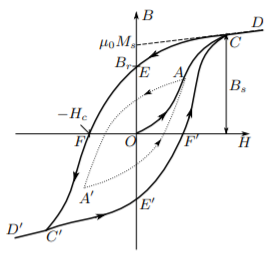
\includegraphics[scale=0.7]{petlya.png}
	\caption{Петля гистерезиса ферромагнетика}
	\label{fig:petlya}
\end{figure}

Магнитная индукция $ B $ и напряжённость поля $ H $ в ферромагнитном материале неоднозначно связаны между собой: индукция зависит
не только от напряжённости, но и от предыстории образца. Связь между $ B $ и $ H $ типичного ферромагнетика иллюстрирует рис. $\ref{fig:petlya}$.

Если к ферромагнитному образцу прикладывать переменное внешнее
магнитное поле, то его состояние на плоскости $ B-H $ будет изменяться
по замкнутой кривой — петле гистерезиса. Размер петли определяется
максимальным значением напряжённости $ H $ в цикле (например, петля $ AA' $,
обозначенная пунктиром на рис. $\ref{fig:petlya}$). Если амплитуда напряжённости достаточно велика, то образец будет периодически достигать насыщения,
что на рисунке соответствует кривой $ CEFC'E'F'C $ (предельная петля
гистерезиса). Пересечение предельной петли с вертикальной осью соответствует остаточной индукции $B_r$, пересечение с горизонтальной осью
— коэрцитивному полю $H_c$. Крайние точки петель, соответствующие амплитудным значениям $ H $ (например, точка $ A $ на рис. $\ref{fig:petlya}$), лежат на начальной кривой намагничивания ($ OAC $). Скорость подъема кривой намагничивания характеризуется дифференциальной магнитной проницаемостью:
\begin{equation}
\mu_{дифф} = \frac{1}{\mu_0} \frac{dB}{dH}
\label{equation_going_up}
\end{equation}

\textbf{Измерение магнитной индукции.} 
В лабораторных условиях для исследования зависимости $B(H)$ ферромагнитных материалов обычно используют образцы тороидальной формы. Если на тор намотать равномерную намагничивающую обмотку (рис. 4.6), то поле $H$ внутри тора на окружности радиуса $R$ будет пропорционально току $I$ в обмотке, а его величину можно рассчитать по теореме о циркуляции вектора $H$:
\begin{equation}
H=\dfrac{IN_{0}}{2\pi R},
\label{equation_for_alena}
\end{equation}
где $N_0$ -- число витков намагничивающей обмотки. напряженность магнитного поля в тороидальном образце зависит от $R$, поэтому при $r \ll R$ мы будем иметь достаточно однородную намагниченность образца.

Магнитную индукцию $ B $ удобно
определять с помощью ЭДС, возникающей при изменении магнитного
потока $ \Phi $ в катушке, намотанной на образец. Пусть катушка c $ N $ витками плотно охватывает образец сечением $ S $, и индукция $ B $ в образце
однородна. Тогда
\begin{equation}
|B|=\frac{1}{SN}\int\mathcal{E} dt.
\label{eq:|B|}
\end{equation}
\begin{wrapfigure}{r}{0.3\linewidth}
	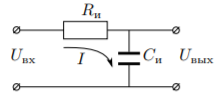
\includegraphics[width=\linewidth]{int.png}
	\caption{Интегрирующая ячейка}
	\label{fig:int}
\end{wrapfigure}

Для интегрирования в работе используется интегрирующая $ RC $-цепочка (рис. $ \ref{fig:int} $).
«Входное» напряжение от источника $U_{\text{вх}}(t)$ подаётся на последовательно соединённые резистор $R_\text{и}$ и конденсатор $C_\text{и}$. <<Выходное>>
напряжение $U_{\text{вых}}(t)$ снимается с конденсатора. Предположим, что 1) сопротивление источника мало по сравнению с $R_\text{и}$, 2) выходное сопротивление (сопротивление на входе осциллографа), напротив, велико: $R_{\text{вых}}$ $ \gg $ $R_\text{и}$ и, наконец, 3) сопротивление $R_\text{и}$ достаточно велико, так что почти всё падение напряжения приходится на него, а $U_{\text{вых}}$ $\ll$ $U_{\text{вх}}$. В таком случае ток цепи равен I = ($U_{\text{вх}}$ - $U_{\text{вых}}$)/$R_\text{и}$ $\approx$ $U_{\text{вх}}$/$R_\text{и}$, и входное и выходное сопротивление связаны соотношением
\begin{equation}
U_{\text{вых}} = \frac{q}{C_\text{и}} = \frac{1}{C_\text{и}}\int\limits_0^t Idt \approx \frac{1}{\tau_\text{и}} \int\limits_0^t U_{\text{вх}}dt,
\label{eq:U_ext}
\end{equation}
где $\tau_\text{и}=R_\text{и}C_\text{и}$ - постоянная времени $ RC $ - цепочки. Для индукции поля из ($\ref{eq:|B|}$) получаем 
\begin{equation}
|B|=\frac{1}{SN}\int U_{\text{вх}} dt=\frac{\tau_\text{и}}{SN}U_{\text{вых}}.
\label{eq:|B|new}
\end{equation}

\textbf{Замечание.} Уточним критерий применимости соотношения ($\ref{eq:U_ext}$). Пусть на вход интегрирующей ячейки подан синусоидальный сигнал с частотой $\omega_0$. Тогда, пользуясь методом комплексных амплитуд, нетрудно найти отношение амплитуд входного и выходного напряжений:
\begin{equation}
\frac{U_{\text{вых}}}{U_{\text{вх}}}=\frac{1/\omega_0C}{\sqrt{R^2+1/(\omega_0C)^2}}.
\end{equation}
Тогда неравенство $U_{\text{вых}} \ll U_{\text{вх}}$ реализуется, если 
\begin{equation}
\tau \equiv RC\gg \frac{1}{\omega_0}
\end{equation}
(импеданс конденсатора мал по сравнению сопротивлением резистора).
В таком случае для синусоидального сигнала имеем
\begin{equation}
\frac{U_{\text{вых}}}{U_{\text{вх}}}\approx\frac{1}{\omega_0\tau}.
\end{equation}
В общем случае, если $\omega_0$ — частота самой низкой гармоники в спектре
произвольного входного сигнала, то при $\omega_0\tau \gg 1$ неравенство $U_{\text{вых}} \ll U_{\text{вх}}$ выполняется на любой частоте $\omega > \omega_0$.


\section{Экспериментальная установка}

Схема установки изображена на рис. $\ref{fig:scheme}$. Напряжение сети (220 В,
50 Гц) с помощью трансформаторного блока Т, состоящего из регулировочного автотрансформатора и разделительного понижающего трансформатора, подаётся на намагничивающую обмотку $N_0$ исследуемого образца.
\begin{figure}[h]
	\centering
	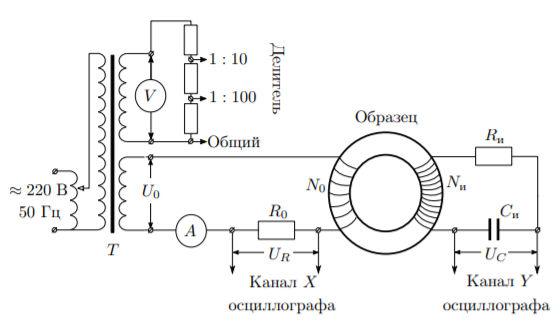
\includegraphics[scale=0.7]{scheme.png}
	\caption{ Схема установки для исследования намагничивания образцов}
	\label{fig:scheme}
\end{figure}
е
В цепь намагничивающей катушки, на которую подаётся некоторое
напряжение $U_0$, последовательно включено сопротивление $R_0$. Напряжение на $R_0$, равное $U_R$= $R_0I_0$, где $I_0$ — ток в намагничивающей обмотке $N_0$, подаётся на канал $ X $ осциллографа. Связь напряжённости $ H $ в
образце и тока $I_0$ рассчитывается по теореме о циркуляции. 
Действующее значение переменного тока в обмотке $N_0$ измеряется амперметром A.
Для измерения магнитной индукции $ B $ с измерительной обмотки $N_\text{и}$
на вход $ RC $-цепочки подаётся напряжение $U_\text{и}$ ($U_{\text{вх}}$), пропорциональное
производной $ dB/dt $. С интегрирующей ёмкости $C_\text{и}$ снимается напряжение $U_C$ ($U_{\text{вых}}$), пропорциональное величине $ B $, и подаётся на вход $ Y $
осциллографа. Значение индукции поля $ B $ рассчитывается по формуле ($\ref{eq:|B|new}$).
Замкнутая кривая, возникающая на экране, воспроизводит в некотором масштабе (различном для осей $ X $ и $ Y $) петлю гистерезиса. Чтобы придать этой кривой количественный смысл, необходимо установить
масштабы изображения, т. е. провести калибровку каналов $ X $ и $ Y $ осциллографа.

 
\section{Ход работы}
\subsection{Измерение петель гистерезиса}

Соберем схему согласно рис. $\ref{fig:scheme}$. Подберем ток питания в намагничивающей обмотке с помощью автотрансформатора и коэффициенты усиления ЭО таким образом, чтобы предельная петля гистерезиса занимала большую часть экрана. Приведем характерные значения катушек разных материалов в таблице \ref{tab:har_kat}.

\begin{table}[h!]
	\centering
	\begin{tabular}{|c|c|c|c|c|}
		\hline
		Материал     & $N_0$ & $N_\text{и}$ & $S^2$, см$^2$ & $2\pi R$, см \\ \hline
		Феррит       & 45    & 400                              & 3,0           & 25,0         \\ \hline
		Пермаллой    & 15    & 300                              & 0,66           & 14,1         \\ \hline
		Крем. железо & 20    & 200                              & 2,0           & 11,0         \\ \hline
	\end{tabular}
	\caption{Характеристики катушек}
	\label{tab:har_kat}
\end{table}

Для каждого образца получим передельные петли гистерезиса, по коэффициентам усиления ЭО $K_x$ и $K_y$ рассчитаем масштабы, определим двойные амплитуды коэрцетивной силы $ [2x(c)] $ и индукции насыщения $ [2y(s)] $. Масштабы по осям $ X $ и $ Y $ рассчитаем по формулам 
$H=IN_0/(2\pi R),\ где\ I=K_x/R_0;\ B=R_\text{и}C_\text{и}U_{\text{вых}}/(SN_\text{и}),$ где $U_{\text{вых}}=K_y$. Результаты измерений и вычислений занесём в таблицы 2,3.

\begin{table}[h!]
	\centering
	\begin{tabular}{|c|c|c|c|c|}
		\hline
		Материал     & $[2x(c)]$, дел & $[2y(s)]$, дел & $K_x$, мВ/дел & $K_y$, мВ/дел \\ \hline
		Феррит       & 3,1            & 2,1            & 20            & 20            \\ \hline
		Пермаллой    & 3,1            & 2,9            & 20            & 100            \\ \hline
		Крем. железо & 1,2            & 2,0            & 20           & 100            \\ \hline
	\end{tabular}
 	\caption{Результаты измерений}

\end{table}

\begin{table}[h!]
	\centering
	\begin{tabular}{|c|c|c|c|}
		\hline
		Материал     & $I_\text{эфф}$, мА & $H$, А$\cdot$м$^{-1}\cdot$дел$^{-1}$ & $B$, Тл/дел \\ \hline
		Феррит       & 253                & $9,3\pm0,9$                        & $0,067\pm0,007 $       \\ \hline
		Пермаллой    & 152                & $10\pm1$                       & $0,095\pm0,001$        \\ \hline
		Крем. железо & 1975                & $120\pm10$                       & $1,10\pm0,12$       \\ \hline
	\end{tabular}
	\caption{Результаты измерений и вычислений}
	\label{tab:izm}
\end{table}

Теперь, зная масштабы по осям, можно определить значения коэрцетивной силы $ H_c $
и индукции насыщения $ B_s $. Результаты заносим в таблицу 4.

\begin{table}[h!]
	\centering
	\begin{tabular}{|c|c|c|c|c|}
		\hline
		Материал     & $H_c$, А/м & $\sigma_{H_c}$, А/м & $B_s$, Тл & $\sigma_{B_s}$, Тл \\ \hline
		Феррит       & 14,4       & 0,8                & 0,143      & 0,005               \\ \hline
		Пермаллой    & 31,0      & 0,9                & 1,45      & 0,07               \\ \hline
		Крем. железо & 69,5      & 1,3                & 1,43      & 0,05               \\ \hline
	\end{tabular}
	\caption{Результаты вычислений}
	\label{tab:vichisl}
\end{table}

Также в следующую таблицу \ref{tab:tab} занесём табличные данные для значений коэрцетивной силы $ H_c $ и индукции насыщения $ B_s $.

\begin{table}[h!]
	\centering
	\begin{tabular}{|c|c|c|}
		\hline
		Материал     & $H_c$, А/м & $B_s$, Тл \\ \hline
		Феррит       & 20         & 0,27      \\ \hline
		Пермаллой    & 11--40     & 1,50--1,52      \\ \hline
		Крем. железо & 80    & 2,0      \\ \hline
	\end{tabular}
	\caption{Табличные данные}
	\label{tab:tab}
\end{table}
Сравнивая полученные данные с табличными можно утверждать, что они совпадают, по крайней мере по порядку величины. Также приведём фотографии предельных петель гистерезиса (рис.4,5,6).

\begin{figure}[h!]
	\centering
	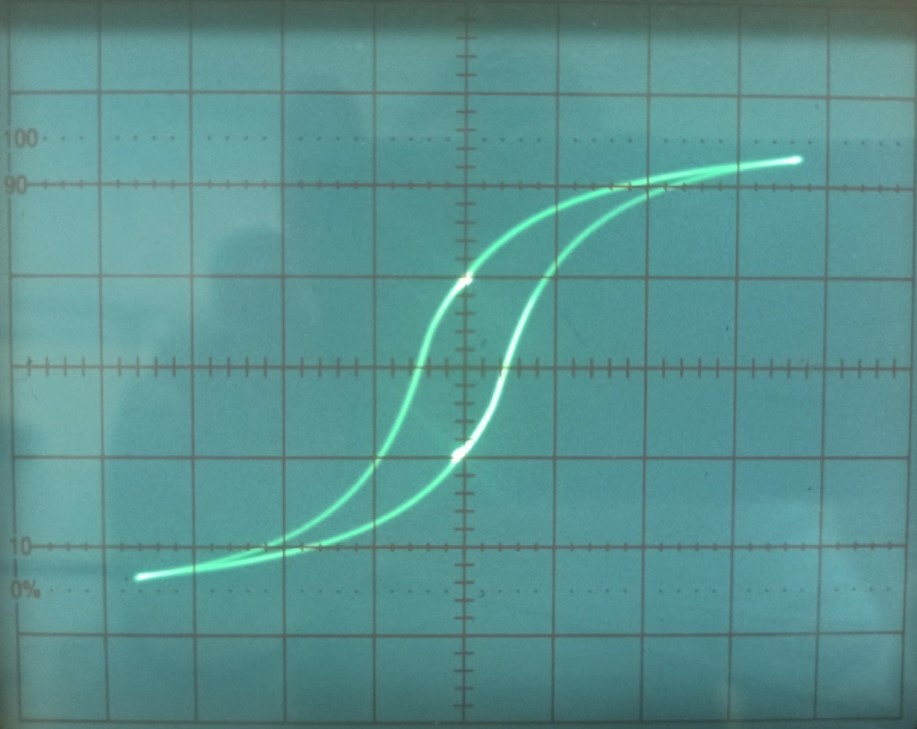
\includegraphics[scale=0.3]{ferrit.jpg}
	\caption{Предельная петля гистерезиса феррита}
\end{figure}
\begin{figure}[h!]
	\centering
	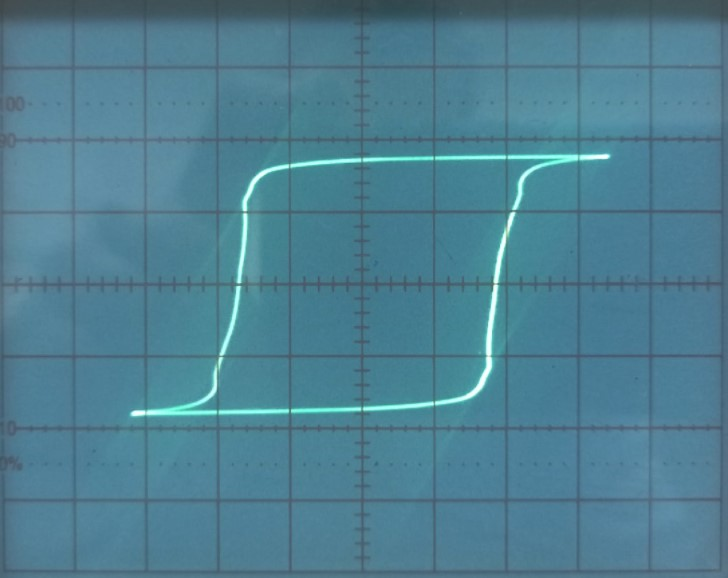
\includegraphics[scale=0.3]{permalloi.jpg}
	\caption{Предельная петля гистерезиса пермаллоя}
\end{figure}
\newpage
\begin{figure}[h!]
	\centering
	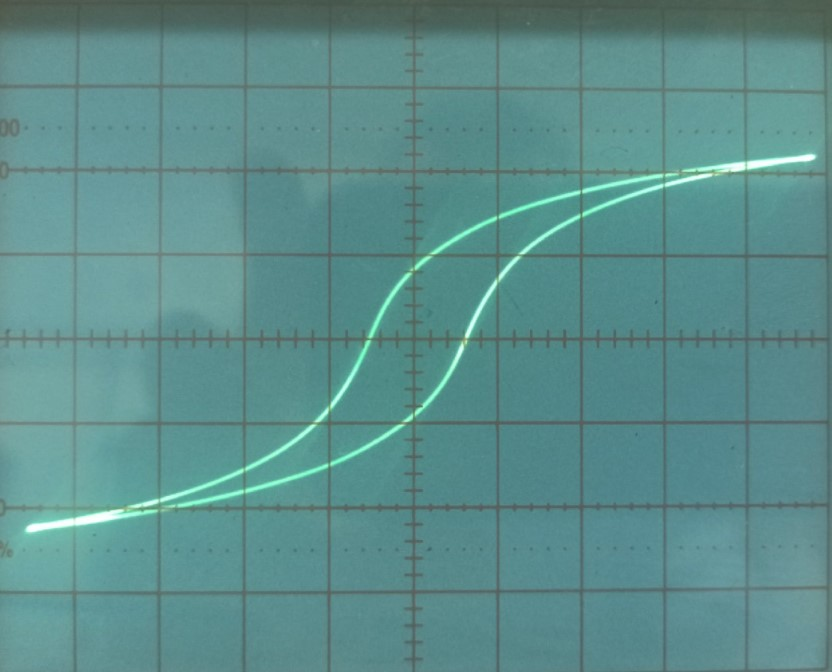
\includegraphics[scale=0.3]{Si_Fe.jpg}
	\caption{Предельная петля гистерезиса для кремнистого железа}
\end{figure}

\subsection{Проверка калибровки осциллографа}

Проверим калибровку ЭО по оси X. Отключим намагничивающую обмотку $N_0$ от цепи, соединив оба провода, идущих к обмотке, на одной ее клемме. С помощью автотрансформатора подберем такой ток через $R_0$, при котором горизонтальная прямая занимает большую часть экрана. При $ K_x=0,1 \text{ В/дел} $ рассчитаем чувствительность $k_x=0,097 \text{ В/дел}$.

Аналогичные действия проводим при $ K_x =0,02 \text{ В/дел} $. Получаем $ k_x=0,019 \text{ В/дел} $.

Так как $k_x \approx K_x$, ЭО откалиброван по оси X корректно.

Также необходимо проверить калибровку по оси $ Y $. Для этого соединим вход Y ЭО с клеммам делителя "1:100 - земля". Не меняя рабочего коэффициента $K_y = 0,05\text{ В/дел}$, подберем с помощью трансформатора напряжение, при котором вертикальная прямая занимает большую часть экрана. Подключим вольтметр V к тем же клеммам делителя и, используя измеренное $U_{\text{эф}}$, рассчитаем чувствительность $k_y=0,048\text{ В/дел}$.

Те же действия повторяем при $K_y = 0,02\text{ В/дел}$. Получаем $k_y=0,017\text{ В/дел}$.

Так как $k_y \approx K_y$, ЭО откалиброван по оси Y корректно.
\subsection{Проверка применимости теоретических выкладок}

Проверим применимость формулы ($\ref{eq:U_ext}$). Для этого рассчитаем $\tau$ -- постоянную времени $ RC $-цепочки. Для определения напряжений на входе и выходе интегрирующей ячейки соединим вход ячейки с обмоткой <<6,3 В>> трансформатора. Подключим Y-вход ЭО ко входу интегрирующей ячейки и отключим X-вход ЭО. Подберем такой ток, чтобы вертикальная прямая занимала большую часть экрана, и определим входное напряжение $U_{\text{вх}}=(0,20\pm0,02) \text{ В}$. Не меняя тока, подключим Y-вход ЭО к выходу ячейки и аналогичным образом определим $U_{\text{вых}}=(0,16\pm0,02) \text{ В}$. Рассчитаем $\tau=\frac{U_{\text{вх}}}{\omega U_{\text{вых}}}=(0,39\pm0,09) \text{ c}$, где $\omega=2\pi\nu$. По определению $\tau_{RC}=R_\text{и}C_\text{и}=0,4\ \text{с}$. Так как $\tau\approx\tau_{RC}$, то условия применимости нашей теории выполнены.
\subsection{Измерение начальной кривой намагничивания}
Проведем измерение начальной кривой намагничивания. Для этого плавно уменьшая амплитуду тока намагничивания до нуля, фиксируем по экрану осциллографа положения крайних точек наблюдаемых петель. Эти вершины лежат на начальной кривой намагничивания. С помощью полученных таким образом графиков оценим максимальные значения дифференциальной магнитной проницаемости и сравним с табличными значениями:

\begin{table}[h!]
\centering
\begin{tabular}{|c|c|c|c|}
\hline
Материал     &    \mu_{dif},\cdot10^3           &     \sigma_{\mu_{dif}},\cdot10^3          & Табличное,\cdot10^3      \\ \hline
Феррит       & 9,0 & 0,5 & 10 \\ \hline
Пермаллой    & 42 & 4 & 3,5-100    \\ \hline
Крем. железо & 8,8 & 0,8 & 7-40     \\ \hline
\end{tabular}
\caption{Значения дифференциальной магнитной проницаемости}
	\label{keklol}
\end{table}

\section{Вывод}
В данной работе изучались петли гистерезиса ферромагнетиков с
помощью электродного осциллографа. По полученным данным
рассчитывались коэрцитивная сила, индукция насыщения и
дифференциальная магнитная проницаемость, совпавшие с табличными
значениями в пределах погрешности и с учетом недостаточной информации о точном составе исследуемых сплавов металлов.
\end{document}

\section{Обработка результатов измерений}


\section{Вывод}


\end{document}
\begin{enumerate}
\subsection{Измерение петель гистерезиса}
\item Собираем схему, подключаем в сеть. Параметры установки $R_\text{и} = 20~\text{кОм}, C_\text{и} = 20~\text{мкФ}, R_0 = 0.2~\text{Ом}$. Параметры образцов:
\begin{table}[h]
\centering
\begin{tabular}{|c|c||c||c|}
\hline
      & Феррит 1000нн & Пермаллой & Кремнистое железо \\ \hline
$N_0$    & 45            & 15        & 20                \\ \hline
$N_\text{и}$    & 400           & 300       & 200               \\ \hline
$S$, см$^2$     & 3.00        & 0.66  & 2.00            \\ \hline
$2\pi R$, cм & 25.0          & 14.1     & 11.0              \\ \hline
\end{tabular}
\end{table}

\item Подбираем ток питания и коэффициенты усиления ЭО так, чтобы предельная петля гистерезиса занимала большую часть экрана. Зарисуем предельную петлю на кальке. Для каждого образца запишем значения коэффициентов усиления $K_{x}$ и $K_{y}$, ток $I_{эф}$. Измерим двойные амплитуды для коэрцитивной силы $2x(c)$ и индукции насыщения $2y(s)$. Результаты:
 	
 	 \begin{itemize}
 	 	\item 	\textbf{Кремниевое железо}:
 	
 	$K_{x}=100 \dfrac{мВ}{дел},$
 	$K_{y}=20 \dfrac{мВ}{дел},$
 	$I_{эф}=1,03 А. $
 	При этом $ 2x = 6,2 дел, \; 2y = 6,8 дел$.
 	
 \item 	\textbf{Пермаллой}:
 	
 	$K_{x}=20 \dfrac{мВ}{дел},$
 	$K_{y}=50 \dfrac{мВ}{дел},$
 	$I_{эф}=218 мА. $
 	При этом $ 2x = 7 дел, \; 2y = 3,5 дел$.
 	
 \item 	 \textbf{Феррит}:
 	 
 $K_{x}=10 \dfrac{мВ}{дел},$
 $K_{y}=50 \dfrac{мВ}{дел},$
 $I_{эф}=92,6 мА. $
 При этом $ 2x = 7,1 дел, \; 2y = 8 дел$.
  	\end{itemize}
\item Восстановим предельные петли для образцов. Рассчитаем  цену деления ЭО для петли для оси Х (в $\dfrac{А}{м}$) по формуле (5), в которой 
 $I=\dfrac{K_{x}}{R_{0}}$, и в Теслах на деление для оси Y по формуле (3), в которой $U_{вых}=K_{y}$:
  	  	
  	  	
  		\begin{itemize}
  			\item \textbf{Кремниевое железо}:
  	  	
  	  	$H=90,9 \dfrac{А}{м}.$
  	  	$B=0,20 \dfrac{Т}{дел}.$
  	
  	\item	\textbf{Пермаллой}:
  	
  $H=10,6 \dfrac{А}{м}.$
  	$B=1,01 \dfrac{Т}{дел}.$
  	
  	\item	\textbf{Феррит}:
  		
  		$H=9,0 \dfrac{А}{м}.$
  		$B=3,33 \cdot 10^{-2} \dfrac{Т}{дел}.$
  	
  		\end{itemize}



\item Снимаем на ту же кальку начальную кривую намагничивания: плавно уменьшая ток намагничивания до нуля, будем отмечать на кальке вершины наблюдаемых частных петель. Кривая, соединяющая эти вершины, проходит вблизи начальной кривой намагничивания. 
\item Восстановим предельную петлю. Измерим на экране двойные амплитуды для коэрцитивной силы и индукции насыщения. Соответствующие значения $K_X$ и $K_Y$.\\
Вычислим цену деления ЭО для петли в А/м по оси Х и в теслах на деление для оси Y.
\item Отключим намагничивающую обмотку от цепи, соединив оба провода, идущих к обмотке, на одной из её клемм. Рассчитаем чувствительность канала X.
\item Разберём цепь тороида. Соединим вход Y ЭО с клеммами делителя "1/100-земля" и подключим вольтметр к тем же точкам делителя. Рассчитаем чувствительность канала X.
\item Для определения напряжений на входе и выходе интегрирующей соединим вход ячейки с обмоткой "6,3 В" трансформатора. 
Подключим Y-вход ЭО ко входу интегрирующей ячейки и отключим Х-вход ЭО. Определим входное напряжение на RC-цепочке:$U_{вх}=2y\cdot K_{y} = 2 \cdot 7,2 = 14,4 $ В.
Не меняя тока, переключим Y-вход ЭО к выходу ячейки  и аналогичным образом определим напряжение  $U_{вых} = 10 \cdot 10^{-3} \cdot 5,6 = 56 \cdot 10^{-3} $ В. Тогда (с учётом $\nu = 50~\text{Гц}$)
\begin{center}
\fbox{$\tau = \dfrac{U_\text{вх}}{\Omega U_\text{вых}} = 0.42 \pm 0.09~\text{с}$}
\end{center}
Рассчитывая через параметры цепи, $\tau = R_\text{и} C_\text{и} = 0.4~\text{c}$, что близко к полученному.

\item  Рассчитаем коэрцитивную силу и индукцию насыщения для каждого образца и сравним с табличными:
\begin{table}[h]
\centering
\begin{tabular}{|c|c|c||c|c||c|c|}
\hline
\multirow{2}{*}{} & \multicolumn{2}{c||}{Феррит 1000нм} & \multicolumn{2}{c||}{Пермаллой} & \multicolumn{2}{c|}{Кремнистое железо} \\ \cline{2-7} 
                  & Значение         & $\sigma$           & Значение       & $\sigma$          & Значение           & $\sigma$              \\ \hline
$H_c$, А/м           & 229         & 11        & 82.0     & 1.6      & 620           & 16          \\ \hline
Таблица           & \multicolumn{2}{c||}{8 - 600}           & \multicolumn{2}{c||}{4}  & \multicolumn{2}{c|}{80}              \\ \hline
$B_s$, Тл            & 0.40              & 0.02        & 4.7 & 0.2      & 0.64               & 0.04         \\ \hline
Таблица           & \multicolumn{2}{c||}{0.2 - 0.4}           & \multicolumn{2}{c||}{1.08}  & \multicolumn{2}{c|}{2.0}              \\ \hline
\end{tabular}
\end{table}
\end{enumerate}